\chapter{Hard- and Softwarestack}\label{ch:hardware-and-softwarestack}


\section{Overview}\label{sec:overview}

The mobile application will be developed for Android and tested using a Google Pixel 7.
The implementation will be carried out in Kotlin using the Android Studio integrated development environment (IDE).

The Google ARCore SDK will be used to access depth information about a scene.
The SDK is available by default -- no additional libraries are required.

Algorithms will be implemented in C\texttt{++} in the \texttt{procedural-augmented-reality} project provided by Prof. Dr. Phillipp Jenke.
This project will be integrated into the application and interfaced with Kotlin through a binding layer.


\section{Google ARCore SDK}

Google's ARCore is a comprehensive Augmented Reality (AR) software development kit (SDK)  for multiple platforms including Android.
It encompasses a broad array of features including motion tracking, anchor tracking, surface tracking, depth perception, and light estimation.
\parencite{arcore}
For the purposes of the topic of this thesis, the depth understanding functionality will be the main focus,
This thesis will primarily utilize ARCore's depth perception capability,
which provides the depth data required for the geometric primitive detection algorithms.

\subsection{Depth API}
Googles documentation~\parencite{arcore-doc-depth} summarizes the features of the Depth API the following way:

\textit{
    The Depth API uses a depth-from-motion algorithm to create depth images, which give a 3D view of the world.
    Each pixel in a depth image is associated with a measurement of how far the scene is from the camera.
    This algorithm takes multiple device images from different angles and compares them to estimate the distance to every pixel as a user moves their phone.
    It selectively uses machine learning to increase depth processing, even with minimal motion from a user.
    It also takes advantage of any additional hardware a user’s device might have.
    If the device has a dedicated depth sensor, such as ToF, the algorithm automatically merges data from all available sources.
}

The development device, Google Pixel 7, does not have a depth sensor.
Consequently, the Depth API will exclusively utilize depth-from-motion techniques to derive depth information from camera images.
However, it is important to note that camera-based depth-from-motion has limitations when it comes to tracking objects with minimal texture, such as walls.
This drawback could potentially present challenges depending on the particular use case being investigated in the thesis.
For instance, if the objective is to recognize objects like boxes or spheres that lack texture, the accuracy of depth information obtained from the Depth API may not be sufficient for accurate recognition.

\subsubsection{API Details}
The Depth API provides two interfaces, as described by \citetitle{arcore-doc-raw-depth}~\parencite{arcore-doc-raw-depth}:
\begin{enumerate}
    \item The Raw Depth API provides "raw depth images that contain a very accurate depth estimate for some, but not all, pixels in the camera image."
    It also provides a "confidence image that gives the confidence for every raw depth images pixel".
    \item The Full Depth API provides a "single 'smoothed' depth image that contains a depth estimate for every pixel."
\end{enumerate}

Example images illustrating the output of the two APIs provided by the Depth API can be seen in figure~\ref{fig:depth-api-images}

The Raw Depth API appears to be the preferable option for the use case of analyzing 3D data, as it provides more accurate data.
The choice between the APIs needs to be investigated further for the final implementation.

\subsubsection{Calculating 3D Point Cloud based on Depth Images}
The Depth API produces depth images instead of point clouds, requiring each pixel to be projected into three-dimensional space using camera intrinsics.
The~\citetitle[p. 5]{arcore-codelab-rawdepth}~\parencite{arcore-codelab-rawdepth} provides a sample implementation called \textit{convertRawDepthImagesTo3dPointBuffer()} which addresses this problem.



\begin{figure}[ht!]
    \centering
    % First row
    \begin{subfigure}[b]{0.4\textwidth}
        \centering
        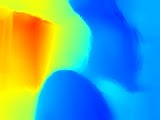
\includegraphics[width=0.8\linewidth]{images/depth_full-depth-image}
        \caption{Full Depth API Depth Image}
    \end{subfigure}%
    \begin{subfigure}[b]{0.4\textwidth}
        \centering
        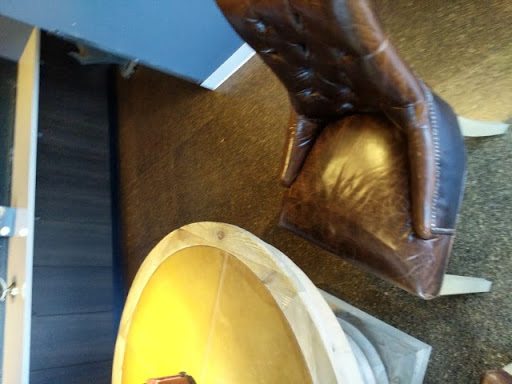
\includegraphics[width=0.8\linewidth]{images/depth_camera-image}
        \caption{Camera image}
    \end{subfigure}%

    % Optional: Adjust or remove vertical spacing between the rows
    \vspace{0.5em}

    % Second row
    \begin{subfigure}[b]{0.4\textwidth}
        \centering
        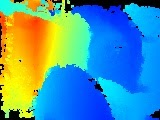
\includegraphics[width=0.8\linewidth]{images/depth_raw-depth-image}
        \caption{Raw Depth API Depth Image}
    \end{subfigure}%
    \begin{subfigure}[b]{0.4\textwidth}
        \centering
        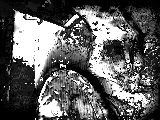
\includegraphics[width=0.8\linewidth]{images/depth_raw-depth-confidence-image}
        \caption{Raw Depth API Confidence Image}
    \end{subfigure}%

    \caption{Full Depth vs. Raw Depth}
    \label{fig:depth-api-images}
\end{figure}

\subsection{Confirming Compatibility with Device}

The quickstart section of the documentation of the \citetitle{arcore-depth-quickstart}~\parencite{arcore-depth-quickstart} provides a sample application named \texttt{hello\_ar\_kotlin}.
The \texttt{hello\_ar\_kotlin} application has been confirmed to run on the hardware mentioned in section~\ref{sec:overview}.
Screenshots of the running sample application can be seen in figure~\ref{fig:hello_world_screenshot}.


\begin{figure}[ht!]
    \centering
    \begin{subfigure}[t]{.45\textwidth}
        \centering
        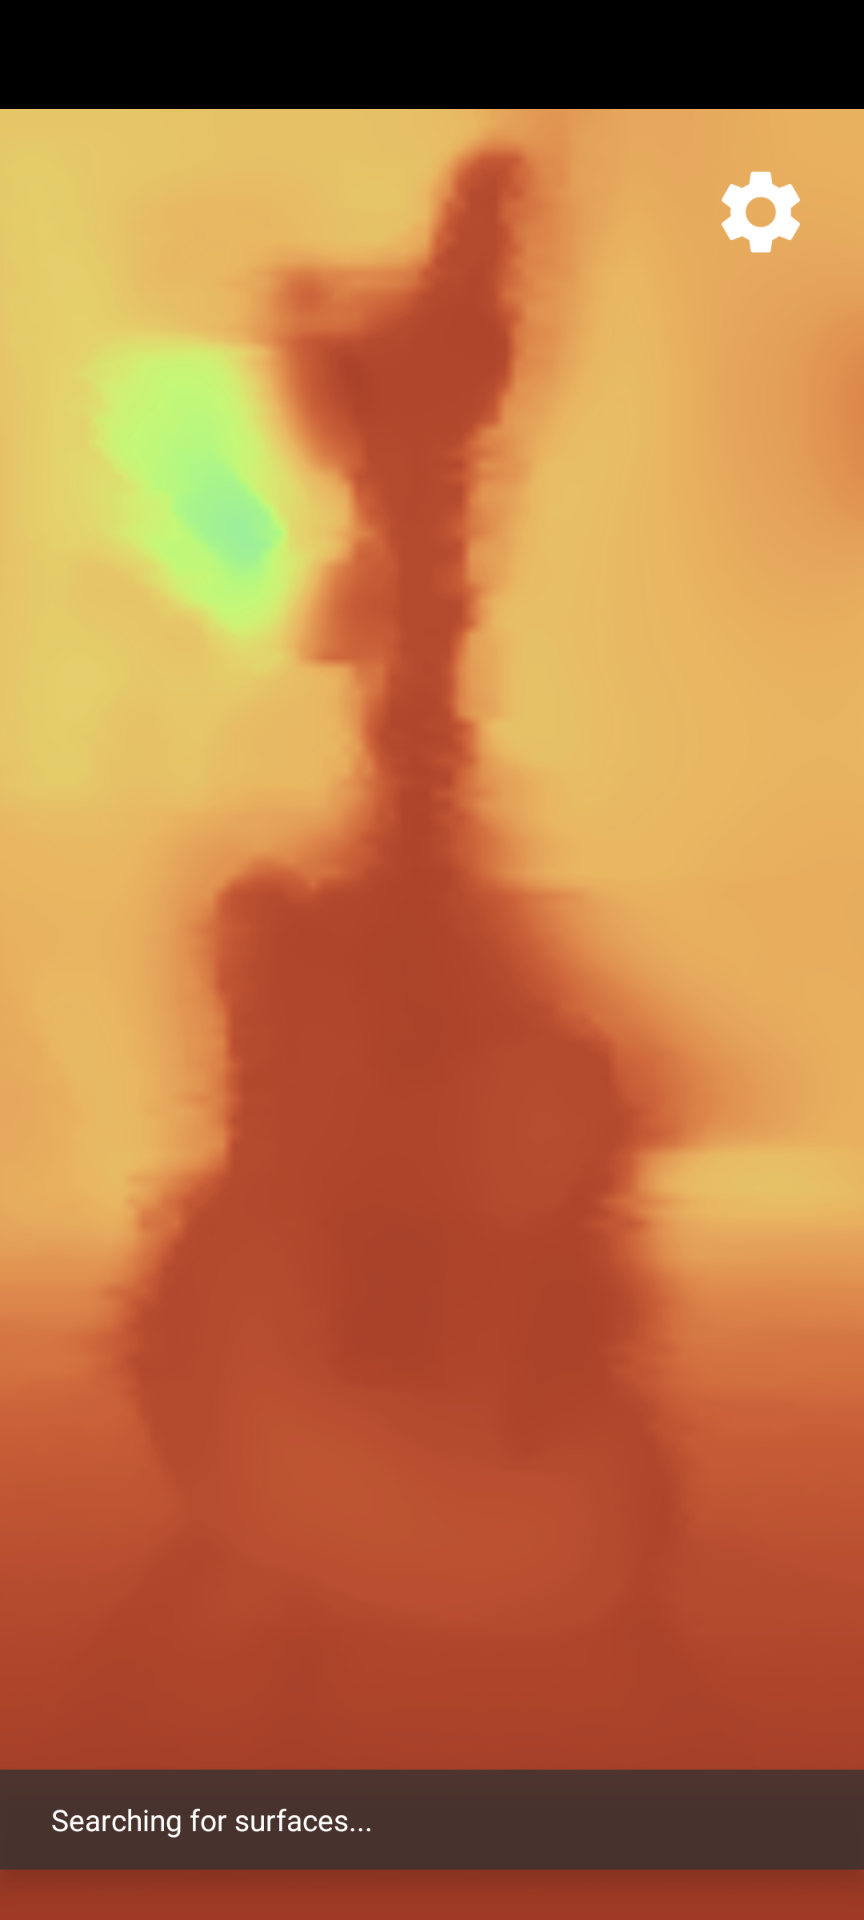
\includegraphics[width=.8\textwidth]{images/depth_api_hello_world_depth}
        \caption{Depth image, colors represent depth}
    \end{subfigure}\hfill
    \begin{subfigure}[t]{.45\textwidth}
        \centering
        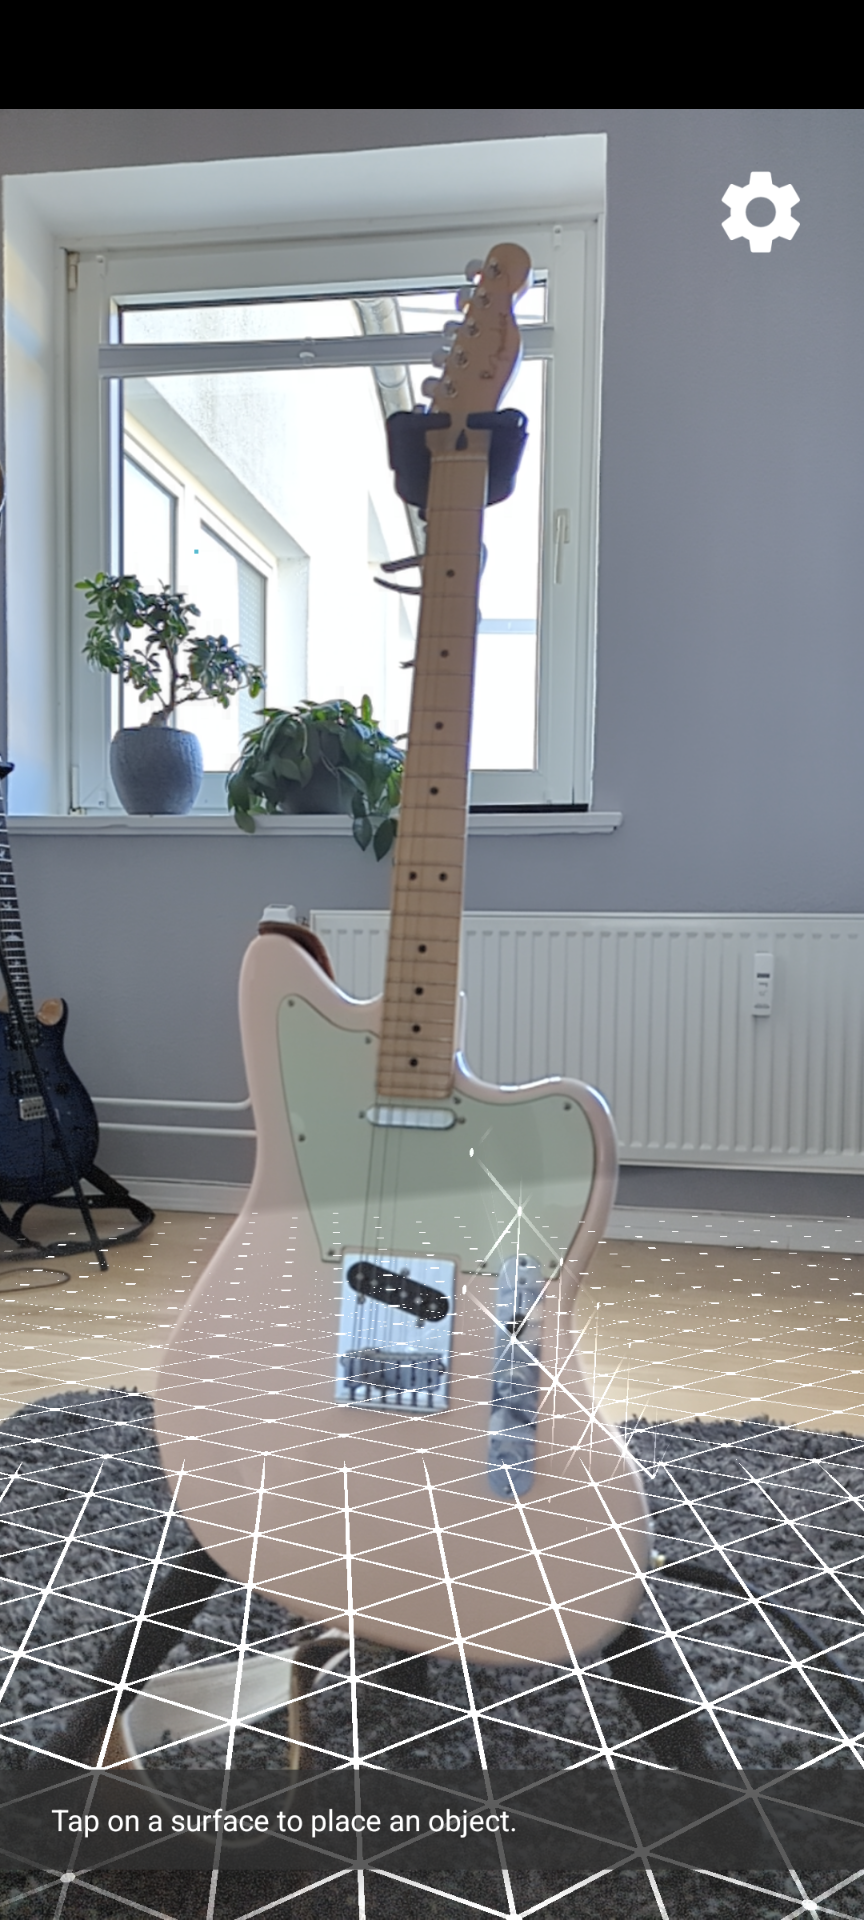
\includegraphics[width=.8\textwidth]{images/depth_api_hello_world_img}
        \caption{Full color reference. Floor is recognized as surface.}
    \end{subfigure}
    \caption{Screenshots of the \texttt{hello\_ar\_kotlin} sample application running on the development device}
    \label{fig:hello_world_screenshot}
\end{figure}
